\chapter{Stratégies Mixtes}

\section{Introduction et Motivation}
Dans certains jeux (ex: tireur vs gardien de but, Pierre-Papier-Ciseaux), l'équilibre en stratégies pures n'existe pas. Si le tireur connaît l'action déterministe du gardien, il peut toujours gagner. L'équilibre réel nécessite de l'aléa, ou plus précisément, de l'imprévisibilité.

\section{Définitions Formelles}

\subsection{Stratégie Mixte et Représentations}
\begin{definition}[Stratégie Mixte]
Une stratégie mixte du joueur $i$ est une mesure de probabilité sur son ensemble d'actions $X_i$.
\begin{itemize}
    \item Si $X_i$ est fini, c'est un vecteur $\sigma_i \in \Delta(X_i) = \{ p \in [0,1]^{|X_i|} : \sum p_k = 1 \}$.
    \item Si $X_i$ est continu (compact), c'est une mesure de probabilité régulière $\mu_i$ sur la tribu de Borel de $X_i$.
\end{itemize}
\end{definition}

\begin{definition}[Vocabulaire Spécifique]
\begin{itemize}
    \item \textbf{Stratégie Pure (Dirac) :} Une stratégie pure $a_i \in X_i$ peut être vue comme une stratégie mixte dégénérée qui met tout le poids sur $a_i$. On la note $\delta_{a_i}$ (mesure de Dirac).
    \item \textbf{Stratégie Totalement Mixte :} Une stratégie mixte $\sigma_i$ est dite \textbf{totalement mixte} si son support est complet, c'est-à-dire si elle assigne une probabilité strictement positive à chaque action pure possible : $\forall x_i \in X_i, \sigma_i(x_i) > 0$.
\end{itemize}
\end{definition}

\paragraph{Triple Représentation :}
Une stratégie mixte peut être vue de trois manières complémentaires :
\begin{enumerate}
    \item \textbf{Géométrique :} Un point dans le simplexe $\Delta(X_i)$.
    \item \textbf{Fonctionnelle :} Une fonction de masse (cas discret) ou de densité.
    \item \textbf{Mesure :} Une mesure de probabilité $\mu$ sur l'ensemble des boréliens.
\end{enumerate}

\begin{center}
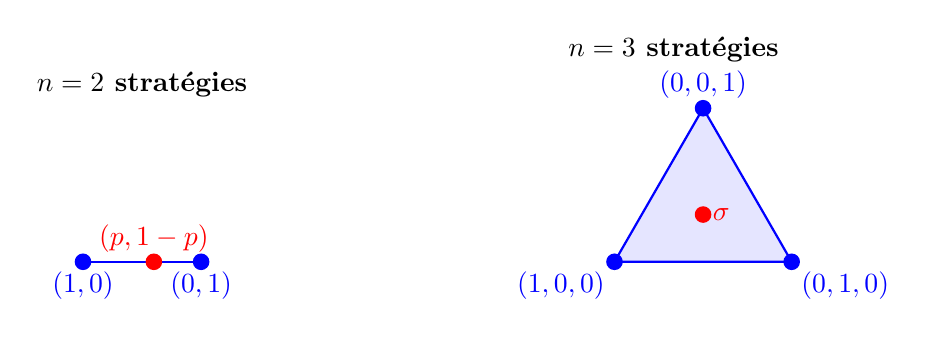
\begin{tikzpicture}[scale=1.5]
    % Simplex for n=2 (segment)
    \begin{scope}[shift={(-2.5,0)}]
        \node at (0.5, 1.5) {\textbf{$n=2$ stratégies}};
        \draw[thick, blue] (0,0) -- (1,0);
        \fill[blue] (0,0) circle (2pt) node[below] {$(1,0)$};
        \fill[blue] (1,0) circle (2pt) node[below] {$(0,1)$};
        \fill[red] (0.6,0) circle (2pt);
        \node[red, above] at (0.6,0) {$(p, 1-p)$};
    \end{scope}
    
    % Simplex for n=3 (triangle)
    \begin{scope}[shift={(2,0)}]
        \node at (0.5, 1.8) {\textbf{$n=3$ stratégies}};
        \coordinate (A) at (0,0);
        \coordinate (B) at (1.5,0);
        \coordinate (C) at (0.75,1.3);
        \draw[thick, blue, fill=blue!10] (A) -- (B) -- (C) -- cycle;
        \fill[blue] (A) circle (2pt) node[below left] {$(1,0,0)$};
        \fill[blue] (B) circle (2pt) node[below right] {$(0,1,0)$};
        \fill[blue] (C) circle (2pt) node[above] {$(0,0,1)$};
        % Interior point
        \fill[red] (0.75,0.4) circle (2pt);
        \node[red, right] at (0.75,0.4) {$\sigma$};
    \end{scope}
\end{tikzpicture}
\captionof{figure}{Le simplexe $\Delta(X_i)$ : segment pour 2 stratégies, triangle pour 3.}
\end{center}

\subsection{Extension Mixte}
L'extension mixte est le "nouveau" jeu où les joueurs choisissent des distributions de probabilité.

\begin{definition}[Gain Espéré et Hypothèse d'Indépendance]
Le gain du joueur $i$ dans l'extension mixte est défini comme l'\textbf{espérance de gain} par rapport à la loi produit des stratégies individuelles.
\textbf{Hypothèse Fondamentale :} Les choix aléatoires des joueurs sont supposés \textbf{indépendants}. Le profil de stratégies mixtes est donc la mesure produit $P = \sigma_1 \otimes \sigma_2 \otimes \dots \otimes \sigma_n$ sur l'espace $X = \prod X_i$.

\textbf{Formulation Intégrale :}
$$\tilde{u}_i(\sigma_1, \dots, \sigma_n) = \int_{X_1} \dots \int_{X_n} u_i(x_1, \dots, x_n) d\sigma_1(x_1) \dots d\sigma_n(x_n)$$

\subsection{Stratégies mixtes en univers continu}
Si l'ensemble des actions $X_i$ est un espace métrique (ex: $[0,1]$), une stratégie mixte $\sigma_i$ est une \textbf{mesure de probabilité borélienne} sur $X_i$.
On note $\Delta(X_i)$ l'ensemble de ces mesures. Le gain espéré est alors :
\[ u_i(\sigma_1, \dots, \sigma_n) = \int_{X_1} \dots \int_{X_n} u_i(x_1, \dots, x_n) d\sigma_1(x_1) \dots d\sigma_n(x_n) \]
Dans le cas fini :
$$\tilde{u}_i(\sigma) = \sum_{x \in X} u_i(x) \left( \prod_{j \in N} \sigma_j(x_j) \right)$$
\end{definition}

\section{Équilibre de Nash en Stratégies Mixtes}

\subsection{Existence et Lien avec le Pur}
\begin{theoreme}[Nash, 1950]
Tout jeu fini possède au moins un équilibre de Nash en stratégies mixtes.
\end{theoreme}

\begin{proposition}[Relation Pur/Mixte]
L'extension mixte est une généralisation cohérente.
Si $x^* = (x^*_1, \dots, x^*_n)$ est un équilibre de Nash en stratégies pures du jeu original, alors le profil de mesures de Dirac $(\delta_{x^*_1}, \dots, \delta_{x^*_n})$ est un équilibre de Nash de l'extension mixte.
\end{proposition}

\subsection{Principe d'Indifférence (Fondamental)}
C'est l'outil principal de calcul des équilibres mixtes.

\begin{proposition}[Principe d'indifférence]
Soit $\sigma^*$ un équilibre de Nash mixte. Pour tout joueur $i$, toute action pure $x_i$ appartenant au \textbf{support} de sa stratégie (c'est-à-dire jouée avec une probabilité positive $\sigma^*_i(x_i) > 0$) doit rapporter le même gain espéré :
$$u_i(x_i, \sigma^*_{-i}) = \max_{a_i \in X_i} u_i(a_i, \sigma^*_{-i}) = \tilde{u}_i(\sigma^*)$$
En d'autres termes, le joueur est \textbf{indifférent} entre toutes les actions qu'il joue réellement. Les actions non jouées rapportent un gain inférieur ou égal.
\end{proposition}

\begin{proof}[Preuve par l'absurde]
Supposons qu'il existe une action $a$ dans le support de $\sigma_i^*$ telle que $u_i(a, \sigma^*_{-i}) < M$, où $M = \max_{z} u_i(z, \sigma^*_{-i})$.
\begin{enumerate}
    \item Soit $b$ une action qui atteint le maximum $M$.
    \item Construisons une nouvelle stratégie $\sigma'_i$ en transférant le poids (la probabilité) $p_a > 0$ de l'action "médiocre" $a$ vers l'action "optimale" $b$.
    \item Le gain espéré devient :
    \begin{align*}
    \tilde{u}_i(\sigma'_i, \sigma^*_{-i}) &= \tilde{u}_i(\sigma^*_i, \sigma^*_{-i}) - p_a \underbrace{u_i(a, \sigma^*_{-i})}_{< M} + p_a \underbrace{u_i(b, \sigma^*_{-i})}_{M} \\
    &> \tilde{u}_i(\sigma^*_i, \sigma^*_{-i})
    \end{align*}
    \item Comme $u_i(b) > u_i(a)$, on a $\tilde{u}_i(\sigma') > \tilde{u}_i(\sigma^*)$.
\end{enumerate}
Ceci contredit le fait que $\sigma^*$ était une meilleure réponse (équilibre de Nash). Donc toutes les actions du support doivent rapporter le maximum $M$.
\end{proof}

\section{Fondements Topologiques et Mesure}
Cette section détaille le cadre mathématique rigoureux nécessaire pour les jeux infinis.

\begin{itemize}
    \item \textbf{Tribu de Borel :} On munit chaque espace d'actions $X_i$ (supposé métrique compact) de sa tribu de Borel $\mathcal{B}(X_i)$, la plus petite $\sigma$-algèbre contenant tous les ouverts.
    \item \textbf{Mesures Régulières :} On considère l'espace $\mathcal{M}(X_i)$ des mesures de probabilité régulières (toute mesure sur un métrique compact est régulière, i.e. approximable par des compacts intérieurement et des ouverts extérieurement).
    \item \textbf{Topologie Faible-* :} La convergence d'une suite de stratégies $\mu_n \to \mu$ est définie par la convergence des intégrales contre toute fonction continue test $f$ :
    $$\forall f \in C^0(X_i, \mathbb{R}), \quad \int_{X_i} f d\mu_n \to \int_{X_i} f d\mu$$
    \item \textbf{Semi-normes :} Cette topologie est induite par la famille de semi-normes $P_f(\mu) = |\int f d\mu|$.
\end{itemize}

\begin{theoreme}[Compacité Faible]
Si $X_i$ est compact métrique, alors l'ensemble des stratégies mixtes $\Delta(X_i)$ est compact pour la topologie faible-*.
\end{theoreme}
C'est ce théorème, combiné à la linéarité (donc quasi-concavité) des gains espérés, qui permet d'appliquer le théorème de Glicksberg pour prouver l'existence d'équilibres dans les jeux continus.

\section{Exemples Classiques}

\begin{exemple}[Exemple de calcul détaillé 2x2]
Considérons le jeu suivant, où le Joueur 1 (lignes) choisit entre $X$ et $Y$, et le Joueur 2 (colonnes) entre $x$ et $y$.
\begin{center}
\begin{tabular}{c|c|c}
 & $x$ ($q$) & $y$ ($1-q$) \\ \hline
$X$ ($p$) & (2, 1) & (0, 0) \\ \hline
$Y$ ($1-p$) & (0, 0) & (1, 2)
\end{tabular}
\end{center}
Le Joueur 1 joue $X$ avec probabilité $p$, le Joueur 2 joue $x$ avec probabilité $q$.

\textbf{Calcul pour le Joueur 1 (Indifférence) :}
Pour que P1 soit disposé à mixer (jouer aléatoirement), il doit être indifférent entre $X$ et $Y$. Ses espérances de gain doivent être égales :
\[ E[U_1(X, \sigma_2)] = E[U_1(Y, \sigma_2)] \]
\[ q \cdot 2 + (1-q) \cdot 0 = q \cdot 0 + (1-q) \cdot 1 \]
\[ 2q = 1 - q \implies 3q = 1 \implies q = 1/3 \]

\textbf{Calcul pour le Joueur 2 (Indifférence) :}
De même, P2 doit être indifférent entre $x$ et $y$ :
\[ E[U_2(\sigma_1, x)] = E[U_2(\sigma_1, y)] \]
\[ p \cdot 1 + (1-p) \cdot 0 = p \cdot 0 + (1-p) \cdot 2 \]
\[ p = 2(1 - p) \implies p = 2 - 2p \implies 3p = 2 \implies p = 2/3 \]

\textbf{Conclusion :} L'unique équilibre de Nash en stratégies mixtes est le profil $((p=2/3), (q=1/3))$.
Graphiquement, les correspondances de meilleure réponse se croisent en ce point $(2/3, 1/3)$ dans le carré des probabilités.
\end{exemple}

\begin{exemple}[Chicken Game]
Indifférence P1 : $-4q + (1-q) = -q \implies q = 1/4$.
\end{exemple}
